\clearpage

\section {Systematic effects in the prediction of the single $\mu$-like ring event reconstructed energy spectrum}
\label{sec:systematics}

%....................................................................................................................
%....................................................................................................................

\subsection {Input systematic parameters}
\label{sec:systematics:inputs}

This analysis considers 48 systematic parameters which can be grouped into 4 categories:
\begin{enumerate}
\item SuperK detector parameters (Sec. \ref{sec:systematics:inputs:superk_det})
\item Correlated flux and cross-section parameters tuned by the BANFF group to ND280 data (Sec. \ref{sec:systematics:inputs:banff})
\item Uncorrelated cross-section parameters (Sec. \ref{sec:systematics:inputs:uncor_xsec})
\item Intranuclear and secondary interactions (Sec. \ref{sec:systematics:inputs:fsi}).
\end{enumerate}
A summary of all systematic parameters considered in this analysis is given in Tab.\ \ \ref{tab:input_uncertainties}.
These systematic parameters are applied to the MC templates as shown in Tab.\ \ \ref{tab:apply_syst_to_templates}.

%
% Summary table with systematic parameters
%

{
\begin{table*}[htb]
\thisfloatpagestyle{empty}
\small
\center
\renewcommand{\arraystretch}{1.75} % enlarge line spacing
\begin{tabular}{p{0.12\textwidth}p{0.65\textwidth}p{0.16\textwidth}}
%
% SuperK
%
\hline
\multicolumn {2}{l} { {\bf SuperK detector systematics} } \\
\hline
\parbox{0.12\textwidth}
{
   $f_{E; r}^{SK}$  
}&
\parbox{0.65\textwidth}
{
    \vspace{0.2cm}
    Reconstructed energy scale \\
}&
\parbox{0.16\textwidth}
{
  2.3\%
}\\
\parbox{0.12\textwidth}
{
   $f_{CCQERCi; r}^{SK}$
}&
\parbox{0.65\textwidth}
{
    \vspace{0.2cm}
    $\nu_\mu$, $\bar{\nu}_{\mu}$ CCQE ring-counting efficiency. 
    Three correlated systematic parameters are included (i=0,1,2) corresponding to different reconstructed energy ranges.
    See Sec.\ref{sec:systematics:inputs:superk_det}.\\
}&
\parbox{0.16\textwidth}
{
    1.7\% ($<$ 0.4 GeV) \\ 
    3.5\% (0.4-1.1 GeV) \\
    9.3\% ($>$ 1.1 GeV) 
}\\
\parbox{0.12\textwidth}
{
   $f_{CCQEoth; r}^{SK}$
}&
\parbox{0.65\textwidth}
{
    \vspace{0.2cm}
    $\nu_\mu$, $\bar{\nu}_{\mu}$ CCQE other (all but ring-counting) efficiency. 
    Includes fiducial volume, reduction chain, OD cut, PID cut, momentum cut and decay electron cut efficiencies. \\
}&
\parbox{0.16\textwidth}
{
  1.8\%
}\\
\parbox{0.12\textwidth}
{
   $f_{CCnonQE; r}^{SK}$
}&
\parbox{0.65\textwidth}
{
    \vspace{0.2cm}
    $\nu_\mu$, $\bar{\nu}_{\mu}$ CCnQE efficiency \\
}&
\parbox{0.16\textwidth}
{
  20\%
}\\
\parbox{0.12\textwidth}
{
   $f_{NC; r}^{SK}$
}&
\parbox{0.65\textwidth}
{
    \vspace{0.2cm}
    NC efficiency \\
}&
\parbox{0.16\textwidth}
{
  111\%
}\\
\parbox{0.12\textwidth}
{
   $f_{\nu_e; r}^{SK}$
}&
\parbox{0.65\textwidth}
{
    \vspace{0.2cm}
    $\nu_e$, $\bar{\nu}_{e}$ efficiency \\
}&
\parbox{0.16\textwidth}
{
  100\%
}\\
%
% BANFF systematics
%
\multicolumn {2}{l} { {\bf Correlated flux and cross-section (BANFF) systematics} } \\
\hline
\parbox{0.12\textwidth}
{ 
   $f_{i; t, r}^{banff}$  
}&
\parbox{0.65\textwidth}
{
    \vspace{0.2cm}
    Flux and cross-section parameters tuned by BANFF group on ND280 data.
    Twenty-three correlated parameters are included (i=0,...,22). 
    See Sec.\ \ref{sec:systematics:inputs:banff}.\\
}&
\parbox{0.16\textwidth}
{
  
}\\
\hline
%
% Neutrino Generator
%
\multicolumn {2}{l} { {\bf Uncorrelated cross-section systematics} } \\
\hline
\parbox{0.12\textwidth}
{ 
    \vspace{0.2cm}
    $f_{pF; t, r}$ 
}&
\parbox{0.65\textwidth}
{
    \vspace{0.2cm}
    Fermi momentum (CCQE only)\\ 
    %Applied to CCQE modes 
   
}&
\parbox{0.16\textwidth}
{
  225$\pm$30 MeV
}\\
\parbox{0.12\textwidth}
{ 
    \vspace{0.2cm}
    $f_{bindE; t, r}$ 
}&
\parbox{0.65\textwidth}
{
    \vspace{0.2cm}
    Binding energy for $^{16}O$ (CCQE only)\\
    %Applied to CCQE modes 
}&
\parbox{0.16\textwidth}
{
  27$\pm$9 MeV
}\\
\parbox{0.12\textwidth}
{ 
    \vspace{0.2cm}
    $f_{SF; t, r}$ 
}&
\parbox{0.65\textwidth}
{
    \vspace{0.2cm}
    Nuclear environment modeling; switch from Fermi Gas (RFG) to Spectral Function (SF) model (CCQE only).\\
}&
\parbox{0.16\textwidth}
{
  0 (RFG) - 1 (SF)
}\\
\parbox{0.12\textwidth}
{ 
    \vspace{0.2cm}
    $f_{\pi-less\Delta; t, r}$ 
}&
\parbox{0.65\textwidth}
{
    \vspace{0.2cm}
    Fraction of $\pi$-less $\Delta$ decays in resonance neutrino-production events\\
}&
\parbox{0.16\textwidth}
{
  20\%
}\\
\parbox{0.12\textwidth}
{ 
    \vspace{0.2cm}
    $f_{CCothShape; t, r}$ 
}&
\parbox{0.65\textwidth}
{
    \vspace{0.2cm}
    Parameterizes the uncertainty in CC multipion, CC DIS and CC resonant $\eta$, K and photon production. \\
}&
\parbox{0.16\textwidth}
{
  40\%
}\\
\parbox{0.12\textwidth}
{ 
    \vspace{0.2cm}
    $f_{Wshape; t, r}$ 
}&
\parbox{0.65\textwidth}
{
    \vspace{0.2cm}
    Modifies the shape of the initial pion momentum distribution (before final-state interactions) in resonance interactions. \\
}&
\parbox{0.16\textwidth}
{
  87.8$\pm$45.3
}\\
\parbox{0.12\textwidth}
{ 
    \vspace{0.2cm}
    $f_{CCcoh; t}$ 
}&
\parbox{0.65\textwidth}
{
    \vspace{0.2cm}
    CC coherent cross-section\\
    %Applied to the corresponding modes 
}&
\parbox{0.16\textwidth}
{
  100\%
   
}\\
\parbox{0.12\textwidth}
{ 
    \vspace{0.2cm}
    $f_{NC1\pi^\pm; t}$ 
}&
\parbox{0.65\textwidth}
{
    \vspace{0.2cm}
    NC1$\pi^\pm$ cross-section\\
    %Applied to the corresponding modes 
   
}&
\parbox{0.16\textwidth}
{
  30\%
}\\
\parbox{0.12\textwidth}
{ 
    \vspace{0.2cm}
    $f_{NCoth; t}$ 
}&
\parbox{0.65\textwidth}
{
    \vspace{0.2cm}
    NC other (all but single $\pi^\pm$) cross-section\\
    %Applied to the corresponding modes 
   
}&
\parbox{0.16\textwidth}
{
  30\%
}\\
\parbox{0.12\textwidth}
{ 
    \vspace{0.2cm}
    $f_{CC\nu_e; t}$ 
}&
\parbox{0.65\textwidth}
{
    \vspace{0.2cm}
    $\nu_e$ / $\nu_\mu$ CC cross-section ratio\\
    %Applied to the CC $\nu_e$ modes only 
   
}&
\parbox{0.16\textwidth}
{
  3\%
}\\
\parbox{0.12\textwidth}
{ 
    \vspace{0.2cm}
    $f_{CC\bar{\nu}; t}$ 
}&
\parbox{0.65\textwidth}
{
    \vspace{0.2cm}
    $\bar{\nu}$ / $\nu$ CC cross-section ratio\\
    %Applied to the CC $\bar{\nu}$ modes only 
   
}&
\parbox{0.16\textwidth}
{
  40\%
}\\
%
% FSI & SI
%
\multicolumn {2}{l} { {\bf FSI+SI systematics} } \\
\hline
\parbox{0.12\textwidth}
{ 
    \vspace{0.2cm}
    $f _{i; r}^{FSI}$ 
}&
\parbox{0.65\textwidth}
{
    \vspace{0.2cm}
    FSI (final state interaction / intranuclear hadron transport) and 
    SI (secondary interaction / detector hadron transport) systematic parameters. 
    Six correlated parameters are included (i=0,...,5) corresponding to different modes and reconstructed energy bins. 
    See Sec. \ref{sec:systematics:inputs:fsi}.\\
}&
\parbox{0.16\textwidth}
{
  
}\\
\hline
\end{tabular}\\[2pt]
\caption{
  Summary table of systematic parameters included the VaLOR $\nu_{\mu}$-disappearance analysis.
  The nuisance parameter symbols used in this paper are shown in the first column.
  An index r in the nuisance parameter symbol denotes dependence on reconstructed energy while an index t denotes 
  dependence on true energy.
  An index i is used where multiple systematic parameters, typically correlated between themselves, are grouped together;
  in these cases we refer you to the main text for the exact parameter definition and for the input covariance matrix.
  Wherever practical, 
  the physics parameter affected by the systematic parameter is shown in the second column
  and the size of the uncertainty is shown in the third column.
}
\label{tab:input_uncertainties}
\end{table*}
}

% ........................................


{
\setlength{\tabcolsep}{3pt}
\renewcommand{\arraystretch}{1.8}
\begin{table}
\tiny
\centering
\begin{tabular}{| c || c | c | c | c | c | c || c | c | c | c | c | c || c | c | c | c | c | c || c | c | c | c | c | c || c | c | c | c |}
\hline
                       & \begin{sideways}   $\nu_{\mu}$ CCQE                   \end{sideways}  &   
                         \begin{sideways}   $\nu_{\mu}$ CC1$\pi$               \end{sideways}  &   
                         \begin{sideways}   $\nu_{\mu}$ CC coherent            \end{sideways}  &   
                         \begin{sideways}   $\nu_{\mu}$ CC other               \end{sideways}  &   
                         \begin{sideways}   $\nu_{\mu}$ NC1$\pi^{\pm}$         \end{sideways}  &  
                         \begin{sideways}   $\nu_{\mu}$ NC other               \end{sideways}  &   
                         \begin{sideways}   $\bar{\nu_{\mu}}$ CCQE             \end{sideways}  &  
                         \begin{sideways}   $\bar{\nu_{\mu}}$ CC1$\pi$         \end{sideways}  &  
                         \begin{sideways}   $\bar{\nu_{\mu}}$ CC coherent      \end{sideways}  &  
                         \begin{sideways}   $\bar{\nu_{\mu}}$ CC other         \end{sideways}  &  
                         \begin{sideways}   $\bar{\nu_{\mu}}$ NC1$\pi^{\pm}$   \end{sideways}  &   
                         \begin{sideways}   $\bar{\nu_{\mu}}$ NC other         \end{sideways}  &   
                         \begin{sideways}   $\nu_{e}$ CCQE                     \end{sideways}  &   
                         \begin{sideways}   $\nu_{e}$ CC1$\pi$                 \end{sideways}  &   
                         \begin{sideways}   $\nu_{e}$ CC coherent              \end{sideways}  &  
                         \begin{sideways}   $\nu_{e}$ CC other                 \end{sideways}  &   
                         \begin{sideways}   $\nu_{e}$ NC1$\pi^{\pm}$           \end{sideways}  &   
                         \begin{sideways}   $\nu_{e}$ NC other                 \end{sideways}  &  
                         \begin{sideways}   $\bar{\nu_{e}}$ CCQE               \end{sideways}  &   
                         \begin{sideways}   $\bar{\nu_{e}}$ CC1$\pi$           \end{sideways}  &   
                         \begin{sideways}   $\bar{\nu_{e}}$ CC coherent        \end{sideways}  &   
                         \begin{sideways}   $\bar{\nu_{e}}$ CC other           \end{sideways}  &  
                         \begin{sideways}   $\bar{\nu_{e}}$ NC1$\pi^{\pm}$     \end{sideways}  & 
                         \begin{sideways}   $\bar{\nu_{e}}$ NC other           \end{sideways}  &   
                         \begin{sideways}   Osc-$\nu_{e}$ CCQE                 \end{sideways}  &   
                         \begin{sideways}   Osc-$\nu_{e}$ CC1$\pi$             \end{sideways}  &   
                         \begin{sideways}   Osc-$\nu_{e}$ CC coherent          \end{sideways}  &   
                         \begin{sideways}   Osc-$\nu_{e}$ CC other             \end{sideways}  \\
\hline
 $f_{E; r}^{SK}$             & \ck & \ck & \ck & \ck & \ck & \ck & \ck & \ck & \ck & \ck & \ck & \ck & \ck & \ck & \ck & \ck & \ck & \ck & \ck & \ck & \ck & \ck & \ck & \ck & \ck & \ck & \ck & \ck  \\
\hline
 $f_{CCQERC0; r}^{SK}$       & \ck &     &     &     &     &     & \ck &     &     &     &     &     &     &     &     &     &     &     &     &     &     &     &     &     &     &     &     &      \\
\hline
 $f_{CCQERC1; r}^{SK}$       & \ck &     &     &     &     &     & \ck &     &     &     &     &     &     &     &     &     &     &     &     &     &     &     &     &     &     &     &     &      \\
\hline
 $f_{CCQERC2; r}^{SK}$       & \ck &     &     &     &     &     & \ck  &     &     &     &     &     &     &     &     &     &     &     &     &     &     &     &     &     &     &     &     &      \\
\hline
 $f_{CCQEoth; r}^{SK}$       & \ck &     &     &     &     &     & \ck  &     &     &     &     &     &     &     &     &     &     &     &     &     &     &     &     &     &     &     &     &      \\
\hline
 $f_{CCnQE; r}^{SK}$         &     & \ck & \ck & \ck &     &     &     & \ck & \ck & \ck &     &     &     &     &     &     &     &     &     &     &     &     &     &     &     &     &     &      \\
\hline
 $f_{NC; r}^{SK}$            &     &     &     &     & \ck & \ck &     &     &     &     & \ck & \ck &     &     &     &     & \ck & \ck &     &     &     &     & \ck & \ck &     &     &     &      \\
\hline
 $f_{\nu_e; r}^{SK}$         &     &     &     &     &     &     &     &     &     &     &     &     & \ck & \ck & \ck & \ck &     &     & \ck & \ck & \ck & \ck &     &     & \ck & \ck & \ck & \ck  \\
\hline
 $f_{0; t, r}^{banff}$       & \ck & \ck & \ck & \ck & \ck & \ck &     &     &     &     &     &     &     &     &     &     &     &     &     &     &     &     &     &     &     &     &     &      \\ 
\hline
 $f_{1; t, r}^{banff}$       & \ck & \ck & \ck & \ck & \ck & \ck &     &     &     &     &     &     &     &     &     &     &     &     &     &     &     &     &     &     &     &     &     &      \\
\hline
 $f_{2; t, r}^{banff}$       & \ck & \ck & \ck & \ck & \ck & \ck &     &     &     &     &     &     &     &     &     &     &     &     &     &     &     &     &     &     &     &     &     &      \\
\hline
 $f_{3; t, r}^{banff}$       & \ck & \ck & \ck & \ck & \ck & \ck &     &     &     &     &     &     &     &     &     &     &     &     &     &     &     &     &     &     &     &     &     &      \\
\hline
 $f_{5; t, r}^{banff}$       & \ck & \ck & \ck & \ck & \ck & \ck &     &     &     &     &     &     &     &     &     &     &     &     &     &     &     &     &     &     &     &     &     &      \\
\hline
 $f_{6; t, r}^{banff}$       & \ck & \ck & \ck & \ck & \ck & \ck &     &     &     &     &     &     &     &     &     &     &     &     &     &     &     &     &     &     &     &     &     &      \\
\hline
 $f_{7; t, r}^{banff}$       & \ck & \ck & \ck & \ck & \ck & \ck &     &     &     &     &     &     &     &     &     &     &     &     &     &     &     &     &     &     &     &     &     &      \\
\hline
 $f_{8; t, r}^{banff}$       & \ck & \ck & \ck & \ck & \ck & \ck &     &     &     &     &     &     &     &     &     &     &     &     &     &     &     &     &     &     &     &     &     &      \\
\hline
 $f_{9; t, r}^{banff}$       & \ck & \ck & \ck & \ck & \ck & \ck &     &     &     &     &     &     &     &     &     &     &     &     &     &     &     &     &     &     &     &     &     &      \\
\hline
 $f_{10; t, r}^{banff}$      & \ck & \ck & \ck & \ck & \ck & \ck &     &     &     &     &     &     &     &     &     &     &     &     &     &     &     &     &     &     &     &     &     &      \\
\hline
 $f_{11; t, r}^{banff}$      &     &     &     &     &     &     & \ck & \ck & \ck & \ck & \ck & \ck &     &     &     &     &     &     &     &     &     &     &     &     &     &     &     &      \\
\hline
 $f_{12; t, r}^{banff}$      &     &     &     &     &     &     & \ck & \ck & \ck & \ck & \ck & \ck &     &     &     &     &     &     &     &     &     &     &     &     &     &     &     &      \\
\hline
 $f_{13; t, r}^{banff}$      &     &     &     &     &     &     & \ck & \ck & \ck & \ck & \ck & \ck &     &     &     &     &     &     &     &     &     &     &     &     &     &     &     &      \\
\hline
 $f_{14; t, r}^{banff}$      &     &     &     &     &     &     & \ck & \ck & \ck & \ck & \ck & \ck &     &     &     &     &     &     &     &     &     &     &     &     &     &     &     &      \\
\hline
 $f_{15; t, r}^{banff}$      &     &     &     &     &     &     & \ck & \ck & \ck & \ck & \ck & \ck &     &     &     &     &     &     &     &     &     &     &     &     &     &     &     &      \\
\hline
 $f_{16; t, r}^{banff}$      & \ck &     &     &     &     &     & \ck &     &     &     &     &     & \ck &     &     &     &     &     & \ck &     &     &     &     &     & \ck &     &     &      \\
\hline
 $f_{17; t, r}^{banff}$      &     & \ck &     & \ck & \ck & \ck &     & \ck &     & \ck & \ck & \ck &     & \ck &     & \ck & \ck & \ck &     & \ck &     & \ck & \ck & \ck &     &\ck  &     & \ck  \\
\hline
 $f_{18; t, r}^{banff}$      & \ck &     &     &     &     &     & \ck &     &     &     &     &     & \ck &     &     &     &     &     & \ck &     &     &     &     &     & \ck &     &     &      \\
\hline
 $f_{19; t, r}^{banff}$      & \ck &     &     &     &     &     & \ck &     &     &     &     &     & \ck &     &     &     &     &     & \ck &     &     &     &     &     & \ck &     &     &      \\
\hline
 $f_{20; t, r}^{banff}$      & \ck &     &     &     &     &     & \ck &     &     &     &     &     & \ck &     &     &     &     &     & \ck &     &     &     &     &     & \ck &     &     &      \\
\hline
 $f_{21; t, r}^{banff}$      &     & \ck &     &     &     &     &     & \ck &     &     &     &     &     & \ck &     &     &     &     &     & \ck &     &     &     &     &     & \ck &     &      \\
\hline
 $f_{22; t, r}^{banff}$      &     & \ck &     &     &     &     &     & \ck &     &     &     &     &     & \ck &     &     &     &     &     & \ck &     &     &     &     &     & \ck &     &      \\
\hline
 $f_{pF; t, r}$              & \ck &     &     &     &     &     & \ck &     &     &     &     &     & \ck &     &     &     &     &     & \ck &     &     &     &     &     & \ck &     &     &      \\
\hline
 $f_{SF; t, r}$              & \ck &     &     &     &     &     & \ck &     &     &     &     &     & \ck &     &     &     &     &     & \ck &     &     &     &     &     & \ck &     &     &      \\
\hline
 $f_{\pi-less\Delta; t, r}$  &     &\ck  &     &     & \ck & \ck &     & \ck &     &     & \ck & \ck &     & \ck &     &     &\ck  &\ck  &     & \ck &     &     & \ck & \ck &     & \ck &     &      \\
\hline
 $f_{bindE; t, r}$           & \ck &     &     &     &     &     & \ck &     &     &     &     &     & \ck &     &     &     &     &     & \ck &     &     &     &     &     & \ck &     &     &      \\
\hline
 $f_{CCothShape; t, r}$      &     &     &     &\ck  &     &     &     &     &     & \ck &     &     &     &     &     & \ck &     &     &     &     &     & \ck &     &     &     &     &     & \ck  \\
\hline
 $f_{Wshape; t, r}$          &     &     &     &     & \ck & \ck &     &     &     &     &\ck  & \ck &     &     &     &     & \ck & \ck &     &     &     &     &\ck  & \ck &     &     &     &      \\
\hline
 $f_{CCcoh; t}$              &     &     & \ck &     &     &     &     &     & \ck &     &     &     &     &     & \ck &     &     &     &     &     & \ck &     &     &     &     &     & \ck &      \\
\hline
 $f_{NC1\pi^\pm; t}$         &     &     &     &     & \ck &     &     &     &     &     & \ck &     &     &     &     &     & \ck &     &     &     &     &     & \ck &     &     &     &     &      \\
\hline
 $f_{NCoth; t}$              &     &     &     &     &     & \ck &     &     &     &     &     & \ck &     &     &     &     &     & \ck &     &     &     &     &     &\ck  &     &     &     &      \\
\hline
 $f_{CC\nu_e; t}$            &     &     &     &     &     &     &     &     &     &     &     &     & \ck & \ck & \ck &\ck  &     &     &\ck  &\ck  & \ck & \ck &     &     & \ck & \ck & \ck & \ck  \\
\hline
 $f_{CC\bar{\nu}; t}$        &     &     &     &     &     &     & \ck & \ck & \ck & \ck &     &     &     &     &     &     &     &     & \ck & \ck & \ck & \ck &     &     &     &     &     &     \\
\hline
 $f _{0; r}^{FSI}$           & \ck &     &     &     &     &     & \ck &     &     &     &     &     &     &     &     &     &     &     &     &     &     &     &     &     &     &     &     &      \\
\hline
 $f _{1; r}^{FSI}$           & \ck &     &     &     &     &     & \ck &     &     &     &     &     &     &     &     &     &     &     &     &     &     &     &     &     &     &     &     &      \\
\hline
 $f _{2; r}^{FSI}$           & \ck &     &     &     &     &     & \ck &     &     &     &     &     &     &     &     &     &     &     &     &     &     &     &     &     &     &     &     &      \\
\hline
 $f _{3; r}^{FSI}$           &     & \ck & \ck & \ck &     &     &     & \ck & \ck & \ck &     &     &     &     &     &     &     &     &     &     &     &     &     &     &     &     &     &      \\
\hline
 $f _{4; r}^{FSI}$           &     &     &     &     &     &     &     &     &     &     &     &     & \ck & \ck & \ck & \ck &     &     & \ck & \ck & \ck & \ck &     &     & \ck & \ck & \ck & \ck  \\
\hline
 $f _{5; r}^{FSI}$           &     &     &     &     & \ck & \ck &     &     &     &     & \ck & \ck &     &     &     &     & \ck & \ck &     &     &     &     & \ck & \ck &     &     &     &      \\
\hline
\end{tabular}
\caption{
  A \ck symbol denotes that the given MC template is modified when the given systematic parameter is tweaked.
  The table lists all 48 systematic parameters considered in this analysis (first column) and 
  all 28 MC templates used for constructing the single $\mu$-like ring event reconstructed energy spectrum p.d.f (first row).
}
\label{tab:apply_syst_to_templates}
\end{table}
}

%\clearpage

%....................................................................................................................
\subsubsection {SuperK detector systematics}
\label{sec:systematics:inputs:superk_det}

The SuperK detector systematics are unchanged from the 2010 analyses \cite{SuperkErrors}. 
They can be broken down into two categories:

\begin{enumerate}
\item Reconstructed energy scale\\ 
  The effect of the uncertainty in the reconstructed energy scale is calculated 
  by scaling the bin edges of the MC templates and,
  assuming uniform distribution of events within the bins, 
  calculating the number of events gained from / lost to neighbouring bins.
  The systematic parameter $f_{E; r}^{SK}$ controls the energy scale
  and its uncertainty is estimated to be 2.3\% \cite{SuperkErrors}.
  The effect of the energy scale uncertainty is propagated to all MC templates as shown in Tab.\ \ref{tab:apply_syst_to_templates}.\\
\item Detector efficiencies\\ 
  Uncertainty in the efficiencies comes from the uncertainties in the fiducial volume and reduction chain, 
  and the OD, ring-counting, PID, momentum and decay-electron cuts.
  The efficiency errors used in this analysis \cite{SuperkErrors} are listed below.
  \begin{itemize}
  \item $\nu_\mu$, $\bar{\nu}_{\mu}$ CCQE:\\
    An energy-dependent ring-counting efficiency error and an 
    energy-independent ``other'' efficiency error (due to all sources of uncertainty other than ring-counting)
    are taken into account.
    For the ring-counting effciciency, we assume correlated errors in 3 $E_{reco}$ bins: 0 - 0.4 GeV, 0.4 - 1.1 GeV and $>$ 1.1 GeV.
    The following error matrix is used:\\
    \\
    $
     \left(
        {\begin{array}{ccc}
           (1.7\%)^2  &   0.59 * 1.7\% * 3.5\%  &  0.33 * 1.7\% * 9.3\% \\
                      &   (3.5\%)^2             &  0.61 * 3.5\% * 9.3\% \\
                      &                         &  (9.3\%)^2            \\
         \end{array} }
     \right)
    $\\
    \\
    For the ``other'' efficiency, we assume an energy-independent error of 1.8\%.
  \item $\nu_\mu$, $\bar{\nu}_{\mu}$ CCnonQE:\\
        A single 20\% energy-independent error is assumed.
        This error was calculated by combining the quoted energy-independent 
        ring-counting (19.9\%) and other (1.7\%) errors in quadrature.
  \item NC:\\
        A single 111\% energy-independent error is assumed.
        This error was calculated by combining the quoted energy-independent 
        ring-counting (48.2\%), PID (100\%) and other (1.7\%) errors in quadrature. 
  \item $\nu_{e}$, $\bar{\nu}_{e}$ CC:\\
        A single $\sim$100\% energy-independent error is assumed.
  \end{itemize}

   The $\nu_\mu$ and $\bar{\nu}_{\mu}$ CCQE ring-counting efficiency is controlled by the systematic parameters
   $f_{CCQERC0; r}^{SK}$ ($E_{reco} <$ 0.4 GeV),
   $f_{CCQERC1; r}^{SK}$ (0.4 GeV $\leq E_{reco} \leq$ 1.1 GeV) and
   $f_{CCQERC2; r}^{SK}$ ($E_{reco} >$ 1.1 GeV), 
   while the ``other'' efficiency is controlled by parameter $f_{CCQEoth; r}^{SK}$.
   The $\nu_\mu$ and $\bar{\nu}_{\mu}$ CCnonQE, the NC and the $\nu_{e}$, $\bar{\nu}_{e}$ CC efficiencies
   are controlled by the systematic parameters
   $f_{CCnQE; r}^{SK}$, $f_{NC; r}^{SK}$ and $f_{\nu_e; r}^{SK}$ respectively.
   These systematic parameters are applied to the MC templates as specified in Tab.\ \ref{tab:apply_syst_to_templates}.
  
\end{enumerate}

\clearpage

%....................................................................................................................
\subsubsection {Correlated flux and cross-section (BANFF) systematics}
\label{sec:systematics:inputs:banff}

The postfit uncertainties of all BANFF flux and cross-section parameters 
and their correlations are taken into account.
A list of the BANFF parameters is given in Tab.\ \ref{tab:banff_params}. 
The BANFF postfit covariance matrix is shown in Fig.\ \ref{fig:banff_postcov},
while both postfit and prefit 1$\sigma$ fractional errors for all parameters
are shown in Fig.\ \ref{fig:banff_postcov_diag_sqrt}. These fractional errors are 
computed from the square roots of the diagonal elements of the corresponding input covariance matrix.

Version 8 of the BANFF matrix is used.

{
\renewcommand{\arraystretch}{1.5}
\begin{table}
\centering
\begin{tabular}{| c | c | c |}
\hline
 Parameter               &  Definition                                                &  Best-fit value (tune v8) \\
\hline
 $f_{0; t, r}^{banff}$   &  $\nu_\mu$ flux normalisation, E = 0.0 - 0.4 GeV           & 0.995 \\
 $f_{1; t, r}^{banff}$   &  $\nu_\mu$ flux normalisation, E = 0.4 - 0.5 GeV           & 1.007 \\
 $f_{2; t, r}^{banff}$   &  $\nu_\mu$ flux normalisation, E = 0.5 - 0.6 GeV           & 1.002 \\
 $f_{3; t, r}^{banff}$   &  $\nu_\mu$ flux normalisation, E = 0.6 - 0.7 GeV           & 0.963 \\
 $f_{4; t, r}^{banff}$   &  $\nu_\mu$ flux normalisation, E = 0.7 - 1.0 GeV           & 0.901 \\
 $f_{5; t, r}^{banff}$   &  $\nu_\mu$ flux normalisation, E = 1.0 - 1.5 GeV           & 0.910 \\
 $f_{6; t, r}^{banff}$   &  $\nu_\mu$ flux normalisation, E = 1.5 - 2.5 GeV           & 0.936 \\
 $f_{7; t, r}^{banff}$   &  $\nu_\mu$ flux normalisation, E = 2.5 - 3.5 GeV           & 0.967 \\
 $f_{8; t, r}^{banff}$   &  $\nu_\mu$ flux normalisation, E = 3.5 - 5.0 GeV           & 0.988 \\
 $f_{9; t, r}^{banff}$  &  $\nu_\mu$ flux normalisation, E = 5.0 - 7.0 GeV            & 0.997 \\
 $f_{10; t, r}^{banff}$  &  $\nu_\mu$ flux normalisation, E = 7.0 - 30.0 GeV          & 1.004 \\
\hline
 $f_{11; t, r}^{banff}$  &  $\bar{\nu}_{\mu}$ flux normalisation, E = 0.0 - 0.7 GeV     & 0.980 \\
 $f_{12; t, r}^{banff}$  &  $\bar{\nu}_{\mu}$ flux normalisation, E = 0.7 - 1.0 GeV     & 0.958 \\
 $f_{13; t, r}^{banff}$  &  $\bar{\nu}_{\mu}$ flux normalisation, E = 1.0 - 1.5 GeV     & 0.947 \\
 $f_{14; t, r}^{banff}$  &  $\bar{\nu}_{\mu}$ flux normalisation, E = 1.5 - 2.5 GeV     & 0.953 \\
 $f_{15; t, r}^{banff}$  &  $\bar{\nu}_{\mu}$ flux normalisation, E = 2.5 -30.0 GeV     & 0.985 \\
\hline
 $f_{16; t, r}^{banff}$  &  CCQE axial mass normalisation, $x_{MAQE}$                             & 1.049 \\
 $f_{17; t, r}^{banff}$  &  Resonant axial mass normation, $x_{MARES}$                        & 1.011 \\
 $f_{18; t, r}^{banff}$  &  CCQE normalisation, E = 0.0 - 1.5 GeV                     & 0.951 \\
 $f_{19; t, r}^{banff}$  &  CCQE normalisation, E = 1.5 - 3.5 GeV                     & 0.708 \\
 $f_{20; t, r}^{banff}$  &  CCQE normalisation, E = 3.5 - 30.0 GeV                    & 1.347 \\
 $f_{21; t, r}^{banff}$  &  CC1$\pi$ normalisation, E = 0.0 - 2.5 GeV                 & 1.370 \\
 $f_{22; t, r}^{banff}$  &  CC1$\pi$ normalisation, E = 2.5 - 30.0 GeV                & 1.016 \\
\hline
\end{tabular}
\caption{
  BANFF parameters and best-fit values (v8 tune) \cite{BANFF}.
}
\label{tab:banff_params}
\end{table}
}

Only the $\nu_\mu$ and $\bar{\nu_\mu}$ flux parameters are included in the BANFF fit.
The $\nu_e$ and $\bar{\nu_e}$ flux parameters have a negligible effect as shown by the results of the systematic study\footnote{
  The study was performed with an older version of the BANFF matrix (v5)} 
in Tab.\ \ref{tab:banff_fluxparams}.

Only those cross-section parameters that are expected to have some cancellation between the ND280 and SuperK are included in the BANFF fit.
The other cross-section parameters included in this analysis are taken to be uncorrelated with the flux parameters
and to have no cancellation between the near and far detectors.
These uncorrelated cross-section parameters are described in Sec.\ \ref{sec:systematics:inputs:uncor_xsec}.

The BANFF parameters are applied to the MC templates as specified in Tab.\ \ref{tab:apply_syst_to_templates}.
All but two of the BANFF cross-section parameters are simple normalization factors.
The parameters $f_{16; t, r}^{banff}$ and $f_{17; t, r}^{banff}$\footnote{
  $f_{16; t, r}^{banff}$ and $f_{17; t, r}^{banff}$ are not the \emph{value} of $M_{A}$, but
  instead a multiplicative factor describing how $M_{A}$ moves away from
  nominal; $M_A$ $\rightarrow$ $x_{MA} M_A$.
} parameterize
the effect of the uncertainty of the axial masses used for modeling CC quasi-elastic 
($M_{A}^{QE}$) 
\footnote{
  An alternative way to treat the quasielastic axial mass was suggested \cite{1overMAQE2}; use 1/$(M_{A}^{QE})^2$ instead of $M_{A}^{QE}$. 
  This is because 1/$(M_{A}^{QE})^2$ has a more linear response than $M_{A}^{QE}$. Distributions of the predicted number of events in SuperK 
  are shown in \cite{Tom1overMaQE2} for 20000 toy experiments with all BANFF matrix parameters randomly thrown for each of these two
  definitions of $M_{A}^{QE}$. Both are Gaussian, suggesting that there is no 
  effect of the $M_{A}^{QE}$ response on the far detector phase space. The shift is thought to be due to the different parameter ranges used: 
  $M_{A}^{QE}$ = 1.21$\pm$0.45 while 1/$(M_{A}^{QE})^2$ = 0.683$\pm$0.320, which translates to $M_{A}^{QE}$ = $1.21^{+0.45}_{−0.21}$. 
  Therefore it was decided to use $M_{A}^{QE}$, to be consistent with the 2012 $\nu_e$ analyses.
} and 
resonance neutrino-production ($M_{A}^{RES}$) 
events respectively;
these have a more complicated, often non-linear, dependence on the true and reconstructed neutrino energy.
Event reweighting methods were used to obtain the fractional changes of the number of events, 
in bins of true and reconstructed neutrino energy, for a range of values (-3.0$\sigma$, -2.5$\sigma$, -2.0$\sigma$, ..., +3.0$\sigma$)
of the $f_{17; t, r}^{banff}$ and $f_{18; t, r}^{banff}$ parameters.
In our p.d.f. calculation, cross-section splines using a polynomial of order 3 are used to interpolate between these event weights 
to obtain the fractional change for any value of these systematic parameters in the (-3.0$\sigma$, +3.0$\sigma$) range.


\begin{table}[htb]
  \centering
  \begin{tabular}{ | l | c c | c c | }
    \hline
    &  \multicolumn {2}{c|} {sin$^2(2\theta_{23})$ = 1.0) }  &  \multicolumn {2}{c|} {sin$^2(2\theta_{23})$ = 0.9} \\
    Systematic & $\delta$ sin$^2(2\theta_{23})$ & $\delta$ $|\Delta m^2_{32}|$  & $\delta$ sin$^2(2\theta_{23})$ & $\delta$ $|\Delta m^2_{32}|$ \\
    \hline
    Statistical & 0.17 & 0.00014 & 0.05 & 0.00022 \\
    \hline
    $\bar{\nu}_{\mu}$ flux 0.0-0.4 GeV & $1 \cdot 10^{-6}$ & $4 \cdot 10^{-7}$ & $5 \cdot 10^{-5}$ & $4 \cdot 10^{-7}$ \\
    $\bar{\nu}_{\mu}$ flux 0.4-0.5 GeV & $1 \cdot 10^{-6}$ & $3 \cdot 10^{-7}$ & $4 \cdot 10^{-5}$ & $4 \cdot 10^{-7}$ \\
    $\bar{\nu}_{\mu}$ flux 0.5-0.6 GeV & $< 1 \cdot 10^{-6}$ & $2 \cdot 10^{-7}$ & $4 \cdot 10^{-5}$ & $2 \cdot 10^{-7}$ \\
    $\bar{\nu}_{\mu}$ flux 0.6-0.7 GeV & $< 1 \cdot 10^{-6}$ & $1 \cdot 10^{-7}$ & $5 \cdot 10^{-5}$ & $2 \cdot 10^{-7}$ \\
    $\bar{\nu}_{\mu}$ flux 0.7-1.0 GeV & $2 \cdot 10^{-6}$ & $4 \cdot 10^{-7}$ & $12 \cdot 10^{-5}$ & $6 \cdot 10^{-7}$ \\
    $\bar{\nu}_{\mu}$ flux 1.0-1.5 GeV & $2 \cdot 10^{-6}$ & $11 \cdot 10^{-7}$ & $12 \cdot 10^{-5}$ & $17 \cdot 10^{-7}$ \\
    $\bar{\nu}_{\mu}$ flux 1.5-2.5 GeV & $1 \cdot 10^{-6}$ & $9 \cdot 10^{-7}$ & $4 \cdot 10^{-5}$ & $15 \cdot 10^{-7}$ \\
    $\bar{\nu}_{\mu}$ flux 2.5-3.5 GeV & $< 1 \cdot 10^{-6}$ & $2 \cdot 10^{-7}$ & $4 \cdot 10^{-5}$ & $2 \cdot 10^{-7}$ \\
    $\bar{\nu}_{\mu}$ flux 3.5-5.0 GeV & $< 1 \cdot 10^{-6}$ & $2 \cdot 10^{-7}$ & $4 \cdot 10^{-5}$ & $2 \cdot 10^{-7}$ \\
    $\bar{\nu}_{\mu}$ flux 5.0-7.0 GeV & $< 1 \cdot 10^{-6}$ & $2 \cdot 10^{-7}$ & $4 \cdot 10^{-5}$ & $2 \cdot 10^{-7}$ \\
    $\bar{\nu}_{\mu}$ flux 7.0-30.0 GeV & $< 1 \cdot 10^{-6}$ & $2 \cdot 10^{-7}$ & $4 \cdot 10^{-5}$ & $2 \cdot 10^{-7}$ \\
    \hline
    $\nu_e$ flux 0.0-0.5 GeV & $< 1 \cdot 10^{-6}$ & $2 \cdot 10^{-7}$ & $4 \cdot 10^{-5}$ & $2 \cdot 10^{-7}$ \\
    $\nu_e$ flux 0.5-0.7 GeV & $< 1 \cdot 10^{-6}$ & $2 \cdot 10^{-7}$ & $4 \cdot 10^{-5}$ & $2 \cdot 10^{-7}$ \\
    $\nu_e$ flux 0.7-0.8 GeV & $< 1 \cdot 10^{-6}$ & $2 \cdot 10^{-7}$ & $4 \cdot 10^{-5}$ & $2 \cdot 10^{-7}$ \\
    $\nu_e$ flux 0.8-1.5 GeV & $< 1 \cdot 10^{-6}$ & $2 \cdot 10^{-7}$ & $4 \cdot 10^{-5}$ & $2 \cdot 10^{-7}$ \\
    $\nu_e$ flux 1.5-2.5 GeV & $< 1 \cdot 10^{-6}$ & $2 \cdot 10^{-7}$ & $4 \cdot 10^{-5}$ & $2 \cdot 10^{-7}$ \\
    $\nu_e$ flux 2.5-4.0 GeV & $< 1 \cdot 10^{-6}$ & $2 \cdot 10^{-7}$ & $4 \cdot 10^{-5}$ & $2 \cdot 10^{-7}$ \\
    $\nu_e$ flux 4.0-30.0 GeV & $< 1 \cdot 10^{-6}$ & $2 \cdot 10^{-7}$ & $4 \cdot 10^{-5}$ & $2 \cdot 10^{-7}$ \\
    \hline
    $\bar{\nu}_{e}$ flux 0.0-2.5 GeV & $< 1 \cdot 10^{-6}$ & $2 \cdot 10^{-7}$ & $4 \cdot 10^{-5}$ & $2 \cdot 10^{-7}$ \\
    $\bar{\nu}_{e}$ flux 2.5-30.0 GeV & $< 1 \cdot 10^{-6}$ & $2 \cdot 10^{-7}$ & $4 \cdot 10^{-5}$ & $2 \cdot 10^{-7}$ \\
    \hline
  \end{tabular}
  \caption{
    Maximum deviation from input values of oscillation parameters for a 2+0 fit and a single parameter $\pm$1 sigma deviation from nominal.
    This uses an old version of the BANFF matrix (v5) with a different parameter set.
    The $\nu_e$ and $\bar{\nu}_{e}$ flux parameters have negligible effect, and they were removed for BANFF v8.
    Similiarly, the first four and last four $\bar{\nu_\mu}$ flux parameters have negligible effect, and these were combined for BANFF v8.
    Made for oscillations with 
    $\sin^22\theta_{12} = $0.857; $\sin^22\theta_{13} = $0.098; $\delta_{CP} = $
    0; $\Delta m^2_{12} = $ 7.5e-05 $eV^{2}/c^{4}$; $|\Delta m^2_{32}| = $ 0.0024 $eV^{2}/c^{4}$
    and  for an exposure of 3.010$\times$10$^{20}$ POT.
  }
  \label{tab:banff_fluxparams}
\end{table}

%
% covariance matrix and errs
%
\begin{figure*}[htb]
\begin{minipage}[t]{0.48\linewidth}
\center
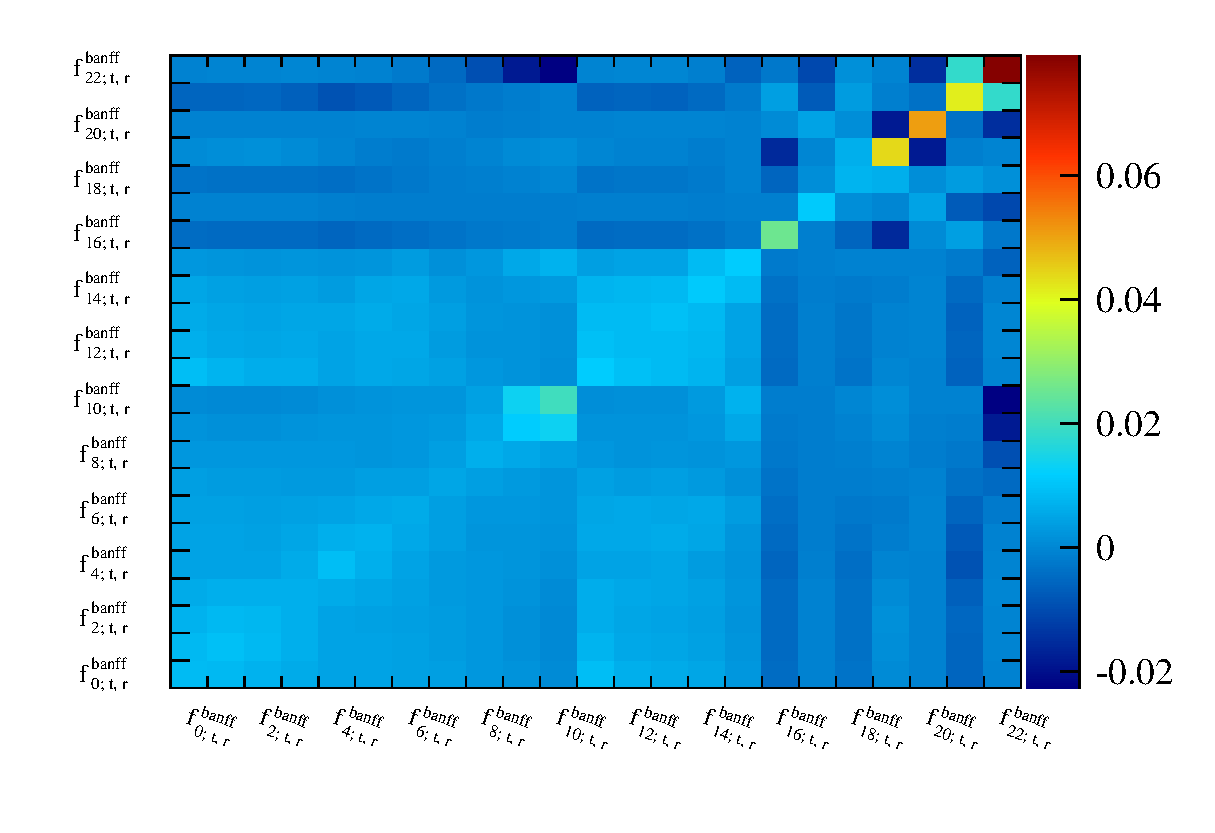
\includegraphics[width=20pc]{./images/spectrum_tweaked/banff}
\caption {
   The input BANFF postfit covariance matrix.
   The meaning of each parameter is given in the text.
}
\label{fig:banff_postcov}
\end{minipage}
\hspace{0.06\linewidth}
\begin{minipage}[t]{0.48\linewidth}
\center
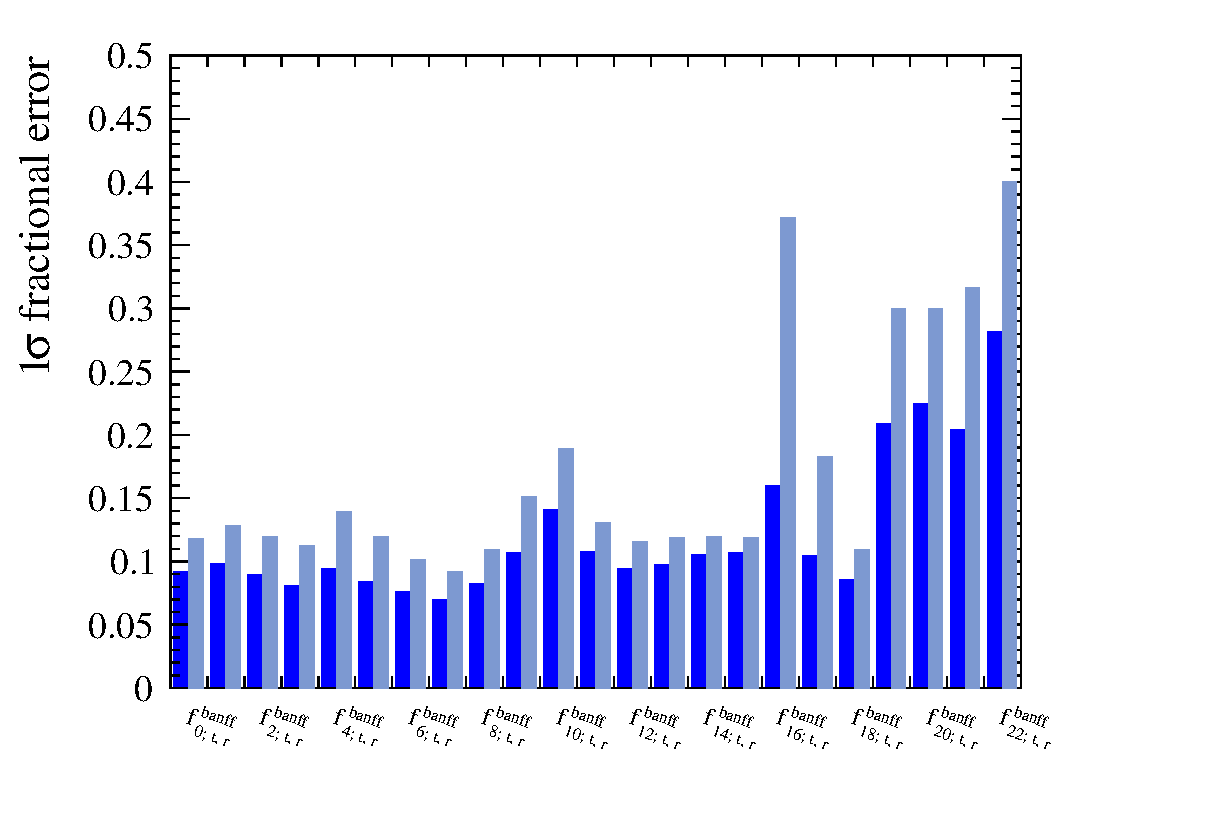
\includegraphics[width=20pc]{./images/spectrum_tweaked/banff_diag_sqrt}
\caption {
   Postfit (dark blue) and prefit (light blue) 1$\sigma$ fractional errors for BANFF parameters
   (computed from the square root of the diagonal elements of the corresponding input covariance matrix).
   The meaning of each parameter is given in the text.
}
\label{fig:banff_postcov_diag_sqrt}
\end{minipage}
\end{figure*}

%....................................................................................................................
\subsubsection {Uncorrelated cross-section systematics}
\label{sec:systematics:inputs:uncor_xsec}

In addition to the BANFF cross-section systematics,
another 11 cross-section systematics are taken into account; these additional systematics are considered to be uncorrelated 
between themselves and to have no cancellation between the near and far detectors \cite{NIWGErr} \cite{MoreNIWGErr113}.

Three of these additional systematics relate to the initial-state nuclear environment modeling for CCQE.
Neutrino Monte Carlo generators typically use Relativistic Fermi Gas (RFG) models,
with or without extensions to take nucleon-nucleon correlation into account, 
and with some, often simplistic, prescription for the treatment of off-shell kinematics.
The RFG model implementation depends on two parameters, the Fermi momentum level (225 MeV for $^{16}O$)
and the nucleon binding energy (27 MeV for $^{16}O$), which are extacted from quasi-elastic electron scattering data.
The systematic parameter $f_{pF; t, r}$ takes into account the effect of a 30 MeV 1$\sigma$ uncertainty in the Fermi momentum level
for $^{16}O$, while parameter $f_{bindE; t, r}$ takes into account the effect of a 9 MeV 1$\sigma$ uncertainty in the nucleon 
binding energy for for $^{16}O$.
The implementation details of the nuclear model can have a significant effect and, therefore,
the effect of switching between two such models was also included as a systematic uncertainty.
This analysis considers the effect of switching between the RFG model and a better-motivated 
Spectral Function (SF) model. The latter does not assume a fixed binding energy and includes the 
correlations between nucleon momentum and binding energy. The systematic parameter $f_{SF; t, r}$ 
includes the effect of switching between the two models.

Simple, energy-independent, generator-level uncertainties are considered for the CC coherent, NC, $\nu_e$ CC
and $\bar{\nu}$ CC cross sections, as the effect of these processes in the single $\mu$-like ring sample is small.
This analysis uses a 100\% uncertainty for the CC coherent cross-section, 
a 30\% uncertainty for both the NC1$\pi^\pm$ and NC ``other'' (all but single $\pi^\pm$) cross section,
a 3\% uncertainty on the $\nu_e$ / $\nu_\mu$ CC cross-section ratio and 
a 40\% uncertainty on the $\bar{\nu}$ / $\nu$ CC cross-section ratio.
The effect of the variation of the above cross sections is included in the analysis
through the systematic parameters $f_{CCcoh; t}$, $f_{NC1\pi^\pm; t}$, $f_{NCoth; t}$,
$f_{CC\nu_e; t}$ and $f_{CC\bar{\nu}; t}$ respectvely.

The treatment of $\Delta$ resonances in the nuclear environment has been controversial in the neutrino
Monte Carlo generator community. Certain models include a ~20\%-level of $\pi$-less $\Delta$ decays in order
to include the effect of $\Delta+N \rightarrow N+N$ scattering, in which the $\Delta$ interacts before it can decay. 
In contrast, other models include no $\pi$-less 
$\Delta$ decays on the basis that this would amount to double counting since, whatever the size of the effect, 
it is already included in hadron-nucleus scattering data to which the intranuclear cascade Monte Carlos are tuned.
This analysis uses NEUT, in which 20\% of $\Delta$s have a $\pi$-less decay by default, and takes the uncertainty in this 
branching fraction to be 100\%. 
The systematic parameter $f_{\pi-less\Delta; t, r}$ includes the effect of varying the fraction of $\pi$-less $\Delta$ 
decays to the corresponding MC templates.

The $f_{CCothShape;t,r}$ systematic parameterizes the uncertainty in CC multi-pion, CC deep inelastic scattering and CC $\eta$, 
K and photon production. From MINOS data, this is known to be $\approx$10\% at 4 GeV. Using this as a reference point, 
the uncertainty is estimated as 0.4/E$_{\nu}$, where E$_{\nu}$ is in GeV. It might appear that this error could diverge at 
low energy, but this does not happen since the threshold is $\approx$0.6 GeV and there are very 
few interactions below 1 GeV. 

The $f_{Wshape;t,r}$ parameter modifies the shape of the initial pion momentum distribution (before final-state interactions) 
by changing the distribution of the pion/nucleon invariant mass while keeping the total cross section constant. As the 
W shape parameter decreases, the pion momentum shifts to lower values, and this increases the probability of pion 
absorption in a final-state interaction. If such an absorption occurs, the event is migrated from CC1$\pi$ (its 
true initial state) and appears to be CCQE.

The effect of the $f_{CCcoh; t}$, $f_{NC1\pi^\pm; t}$, $f_{NCoth; t}$, $f_{CC\nu_e; t}$ and $f_{CC\bar{\nu}; t}$ 
systematic parameters is a simple normalisation change for the corresponding MC templates and thus easily implemented.
Systematic parameters $f_{pF; t, r}$, $f_{SF; t, r}$, $f_{bindE; t, r}$, $f_{\pi-less\Delta; t, r}$, $f_{CCothShape; t, r}$ 
and $f_{Wshape; t, r}$  have a complicated, often non-linear, dependance on true and reconstructed energy.
These are treated in a similar way to the BANFF parameters $f_{17; t, r}^{banff}$ and $f_{18; t, r}^{banff}$ (see Sec.\ 
\ref{sec:systematics:inputs:banff}).
Event reweighting methods were used to obtain the fractional changes of the number of events, 
in bins of true and reconstructed neutrino energy, for a range of values (-3.0$\sigma$, -2.5$\sigma$, -2.0$\sigma$, ..., +3.0$\sigma$)
of the systematic parameters. Again cross-section splines with polynomials of order 3 were used to interpolate between these event 
weights to obtain the fractional change for any
value of these systematic parameters in the (-3.0$\sigma$, +3.0$\sigma$) range.

Some of these systematics are special cases:
\begin{itemize}
\item 
  $f_{SF; t, r}$ is discrete; it can be either off (RFG) or on (SF). 
  Splines are generated with off as nominal, and on as +1.0 sigma.
  Linear interpolation is done only between the weights for 0 and 1.
\item 
  For $f_{Wshape; t, r}$ only $\pm$1.0 sigma errors are evaluated using event reweighting. 
  All other errors are extrapolated or interpolated from these $\pm$1.0 weights.
\item 
  For $f_{\\pi-less\\Delta; t, r}$ only $\pm$1.0 sigma errors are evaluated using event reweighting.
  Weights for tweaks more positive than +1$\sigma$ are extrapolated from the +1$\sigma$ weight. Weights more negative than 
  -1$\sigma$ are taken to be the same as the -1$\sigma$ weight; this is done since 20\% of deltas have a piless decay by 
  default in NEUT, and the error is 20\%. For this reason, it is unphysical to tweak $f_{\\pi-less\\Delta; t, r}$ to be 
  more negative than -1$\sigma$. 
\end{itemize}

The cross-section splines have 41 bins in reconstructed energy:
\begin{itemize}
\item 1 bin from 0-0.3 GeV
\item 14 50-MeV bins from 0.3-1.0 GeV
\item 20 100MeV bins from 1.0-3.0 GeV
\item 2 500-MeV bins from 3.0-4.0 GeV
\item 1 bin from 4.0-5.0 GeV
\item 1 bin from 5.0-7.0 GeV
\item 1 bin from 7.0-10.0 GeV
\item 1 bin from 10.0-30.0 GeV
\end{itemize}
For the $\nu_{\mu}$, $\bar{\nu}_{\mu}$ and oscillated $\nu_{e}$ samples, they have 11 bins in true energy:
\begin{itemize}
\item 1 bin from 0-0.4 GeV
\item 3 100-MeV bins from 0.4-0.7 GeV
\item 1 bin from 0.7-1.0 GeV
\item 1 bin from 1.0-1.5 GeV
\item 2 1-GeV bins from 1.5-3.5 GeV
\item 1 bin from 3.5-5.0 GeV
\item 1 bin from 5.0-7.0 GeV
\item 1 bin from 7.0-30.0 GeV  
\end{itemize}
For the $\nu_{e}$ sample, they have 7 bins in true energy:
\begin{itemize}
\item 1 bin from 0-0.05 GeV
\item 1 bin from 0.5-0.7 GeV
\item 1 bin from 0.7-0.8 GeV
\item 1 bin from 0.8-1.5 GeV
\item 1 bin from 1.5-2.5 GeV
\item 1 bin from 2.5-4.0 GeV
\item 1 bin from 4.0-30.0 GeV 
\end{itemize}
Finally, for the $\bar{\nu}_{e}$ sample, they have 2 bins in true energy:
\begin{itemize}
\item 1 bin from 0-2.5 GeV
\item 1 bin from 2.5-30.0 GeV
\end{itemize}

An example of a cross-section spline is shown in Fig.\ \ref{fig:example_spline}. 

\begin{figure}[htb]
\center
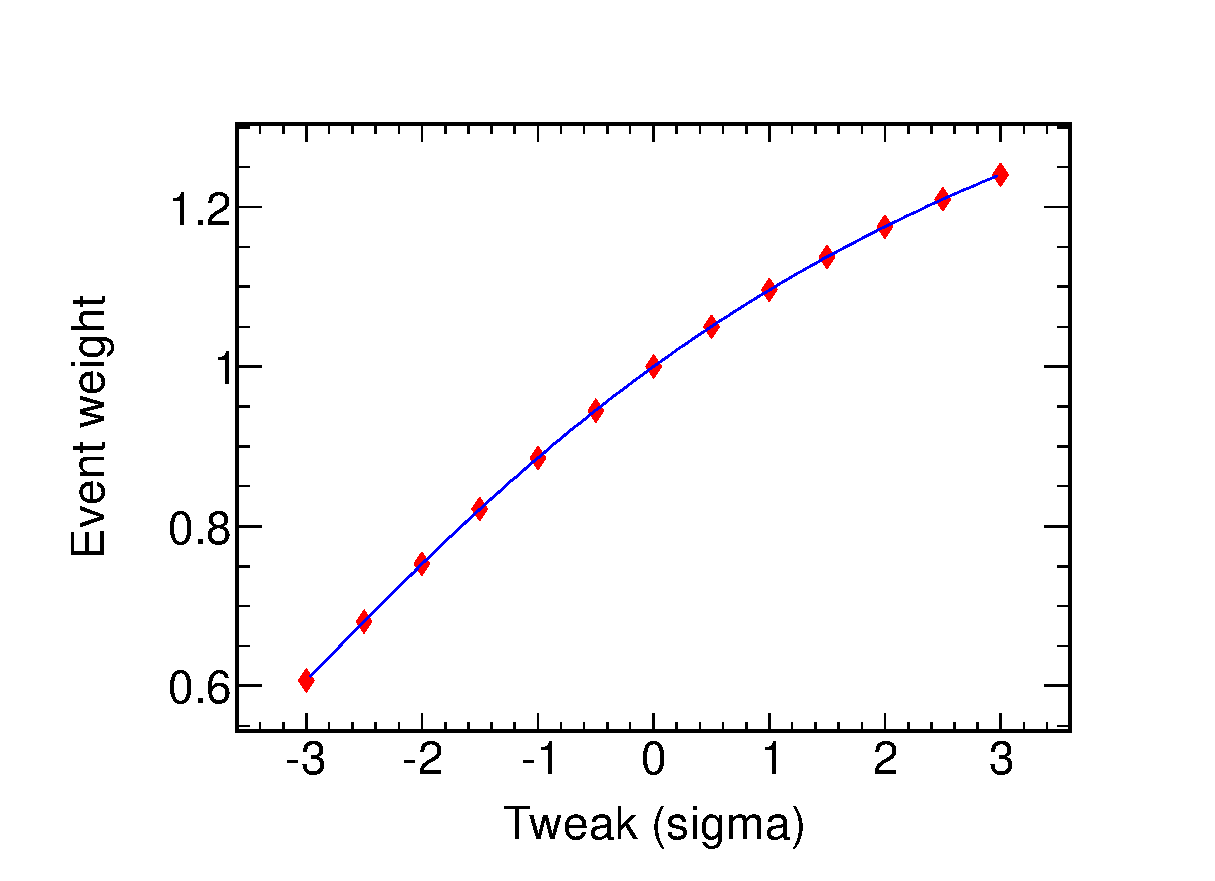
\includegraphics[width=25pc]{./images/spectrum_tweaked/ExampleSpline}
\caption {
Example of a cross-section spline; this shows the event weights obtained by tweaking $M_{A}^{QE}$
for $\nu_{\mu}$-CCQE events in the bin with reconstructed energy 0.75-0.8 GeV and 
true energy 0.6-0.7 GeV.
}
\label{fig:example_spline}
\end{figure}


The 11 uncorrelated cross-section systematics considered in this analysis are summarised in Tab.\ \ref{tab:input_uncertainties}.
These cross-section systematics are applied to the MC templates as shown in Tab.\ \ref{tab:apply_syst_to_templates}.


%....................................................................................................................
\subsubsection {FSI+SI systematics}
\label{sec:systematics:inputs:fsi}

Intranuclear hadron transport, or final-state interactions (FSI),
have significant effects in the T2K energy range and
result in event topologies, for scattering on nuclear targets, which are drastically different
compared with those created in neutrino scattering on free nucleons.
Elastic and inelastic hadron rescattering, secondary pion production, single and double charge exchange
and absorption followed by multi-nucleon knockout are typically modelled in neutrino event generators using
intranuclear cascades.

Uncertainties due to FSI were estimated by simultaneously varying the NEUT parameters that scale the interaction probabilities for quasi-elastic 
scattering, absorption, charge exchange and pion production using the method described in Sec.\ 2 in \cite{NIWGErr}. The NIWG group produced 16 
parameter sets that span the 1$\sigma$ surface in the parameter space; this was done by varying the NEUT parameters when running the pion scattering 
simulations, and comparing the results with external pion-carbon scattering data. These 16 parameter sets are shown in Tab.\ 2 in \cite{NIWGErr}. 

Uncertainties due to secondary pion interactions (SI) were also evaluated. The NIWG group adapted the NEUT nuclear cascade model to simulate SI in the 
SuperK detector simulation (SKDETSIM) and to allow variations in the interaction probabilities. Details of this are given in \cite{SI}. The original 
11c SKMC files do not contain all the truth information required for reweighting SI, and a second production was made. The two productions contain 
independent steps (SKDETSIM was rerun on the NEUT files), and there are small differences in the numbers of events between the productions. The second 
production was used only to produce the FSI+SI covariance matrix, which is shown in Fig.\ \ref{fig:fsi_covmatrix}. 
The 1$\sigma$ fractional errors in the 6 FSI+SI parameters are shown in Fig.\ \ref{fig:fsi_covmatrix_diag_sqrt}; these are computed from the square 
roots of the diagonal elements of the input covariance matrix.

Since the same model is used for FSI and SI, it is possible to evaluate the uncertainties in both FSI and SI simultaneously. This was done by 
reweighting a single $\mu$-like ring selected SK MC with the 16 FSI parameter sets using T2KReweight. The reweighting method for FSI is described 
in Sec. 8 in \cite{NEUTnuclear}. Variations in the SI interaction probabilities were included for each FSI parameter set.  Subsequently a covariance 
matrix was calculated using equation 1 in \cite{NIWGErr}; the quantity p in that equation is the average event weight for a FSI parameter set, and 
the sum is over the parameter sets.

The covariance matrix was made with a 6-bin scheme, as shown in Tab.\ \ref{tab:fsi_si_params}.
For $\nu_\mu$, $\bar{\nu}_{\mu}$ CCQE, the FSI+SI binning scheme
is identical to that used by SuperK for calculating the $\nu_\mu$, $\bar{\nu}_{\mu}$ CCQE ring-counting efficiency error matrix.

{
\renewcommand{\arraystretch}{1.5}
\begin{table}
\centering
\begin{tabular}{| c | c |}
\hline
 Parameter               &  Definition \\
\hline
 $f _{0; r}^{FSI}$       &  $\nu_\mu$ \& $\bar{\nu}_{\mu}$ CCQE, $E_{reco}<$ 0.4 GeV  \\
 $f _{1; r}^{FSI}$       &  $\nu_\mu$ \& $\bar{\nu}_{\mu}$ CCQE, 0.4 GeV $\leq E_{reco} \leq$ 1.1 GeV \\
 $f _{2; r}^{FSI}$       &  $\nu_\mu$ \& $\bar{\nu}_{\mu}$ CCQE, $E_{reco}>$ 1.1 GeV \\
 $f _{3; r}^{FSI}$       &  $\nu_\mu$ \& $\bar{\nu}_{\mu}$ CCnonQE \\
 $f _{4; r}^{FSI}$       &  $\nu_e$, $\bar{\nu}_{e}$ CC \\
 $f _{5; r}^{FSI}$       &  All NC \\
\hline
\end{tabular}
\caption{
  FSI+SI systematic parameters.
}
\label{tab:fsi_si_params}
\end{table}
}

%
% Input FSI param covariance & errs
%
\begin{figure*}[htb]
\begin{minipage}[t]{0.48\linewidth}
\center
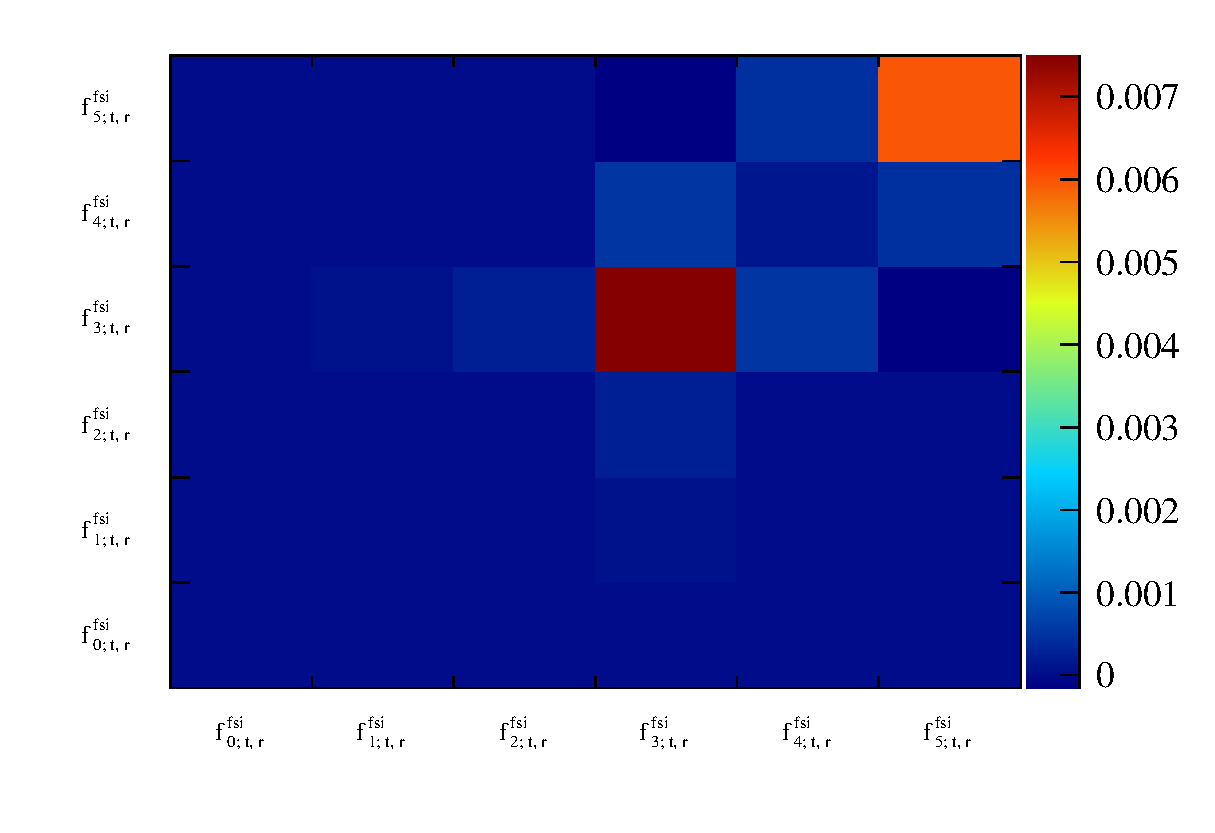
\includegraphics[width=20pc]{./images/spectrum_tweaked/fsi}
\caption {
  The input FSI+SI covariance matrix.
  The meaning of each parameter is given in Tab.\ \ref{tab:fsi_si_params}.
}
\label{fig:fsi_covmatrix}
\end{minipage}
\hspace{0.06\linewidth}
\begin{minipage}[t]{0.48\linewidth}
\center
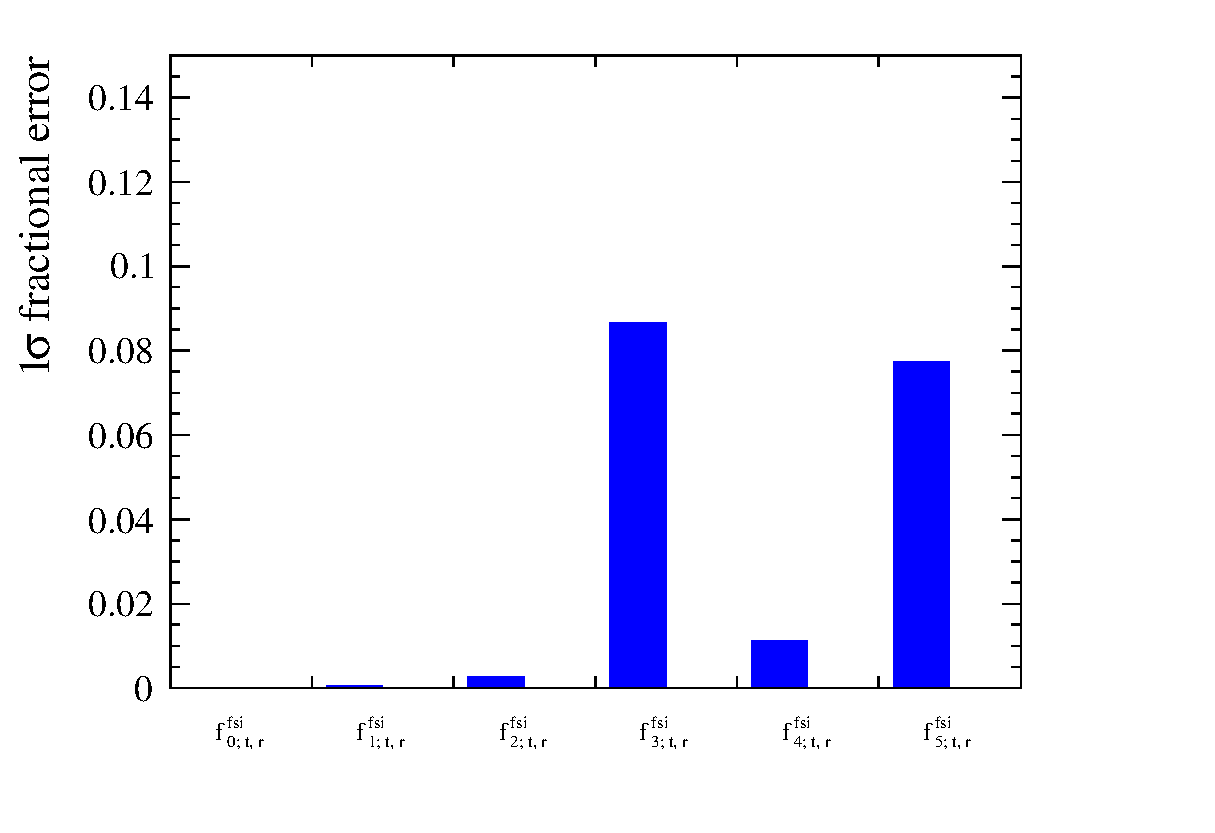
\includegraphics[width=20pc]{./images/spectrum_tweaked/fsi_diag_sqrt}
\caption {
   1$\sigma$ fractional error for FSI+SI parameters
   (computed from the square roots of the diagonal elements of the input covariance matrix).
  The meaning of each parameter is given in Tab.\ \ref{tab:fsi_si_params}.
}
\label{fig:fsi_covmatrix_diag_sqrt}
\end{minipage}
\end{figure*}

%....................................................................................................................
%....................................................................................................................

\subsection {Evaluation of systematic effects on the single $\mu$-like ring reconstructed energy spectrum}
\label{sec:systematics:evaluation}

In this section, we present the effects of the systematics described in Secs.\ \ref{sec:systematics:inputs:banff}, 
\ref{sec:systematics:inputs:uncor_xsec} and \ref{sec:systematics:inputs:fsi} on the expected 
number of single $\mu$-like ring events and the reconstructed energy spectrum in SuperK.
These effects are shown both for no oscillations and for oscillations with
$\sin^{2}2\theta_{23}$ = 1.0 and $|\Delta m^{2}_{32}|$ = 2.4$\times10^{-3}$ $eV^{2}/c^{4}$.
For the oscillation cases, the 2012 PDG values are used for $\sin^{2}2\theta_{13}$, $\sin^{2}2\theta_{12}$ and $\Delta m^{2}_{21}$,
and $\delta_{CP}$=0. The normal mass hierarchy is assumed.
All results are generated for an integrated exposure of 3.010$\times$10$^{20}$ POT and
the BANFF-tuned MC templates are used.

The effects of systematic uncertainties on the expected number of events, both for no oscillations and for oscillations 
with the typical parameter values given above, is summarised in Tab.\ \ref{tab:nsk_systematic_table_summary}.
In this table, systematic parameters are grouped into a few categories and all parameter correlations are taken into account.
Entries for both the BANFF prefit and postfit errors are provided.
The effects of each parameter individually are presented in Tab.\ \ref{tab:nsk_systematic_table} in which the correlations 
between parameters are necessarily ignored.

The effects of the combined systematic uncertainties on the reconstructed energy spectrum of single $\mu$-like ring events
is shown in Fig.\ \ref{fig:1Rmu_error_envelope_total}, for the typical oscillation scenario used.
This plot shows the total error envelope for the 1 $\mu$-like ring event reconstructed energy spectrum; this is calculated 
as the $\pm$1$\sigma$ spread of bin contents from 100k toy MC experiments generated with randomized systematic parameters.
In Fig.\ \ref{fig:1Rmu_error_envelope_total}, all systematic parameters were considered and their correlations were taken 
into account.

Error envelopes from the effects of certain groups of systematic parameters are shown in  
Figs.\ \ref{fig:1Rmu_error_envelope_superk_det} (SuperK detector systematics only), 
\ref{fig:1Rmu_error_envelope_banff} (BANFF systematics only), 
\ref{fig:1Rmu_error_envelope_uncor_xsec} (uncorrelated cross-section systematics only), and 
\ref{fig:1Rmu_error_envelope_fsi} (FSI+SI systematics only).

Detailed studies showing the effects of individual systematics on the expected number of
single $\mu$-like ring events are shown in Appendix \ref{appendix:nsk_systematics},
while their effects on the reconstructed energy spectrum of the single $\mu$-like ring sample
are shown in Appendix \ref{appendix:spectrum_systematics}.

%..................

\begin{table}
\centering
\begin{tabular}{| c | c | c |}
\hline
  {\bf Source of uncertainty}  &  {\bf ${\delta}N_{SK}$/$N_{SK}$}  & {\bf ${\delta}N_{SK}$/$N_{SK}$} \\
                               &  (no oscillation)                 & (oscillations with typical parameter values) \\
\hline
SuperK detector       &  5.57\%   & 10.08\%  \\
BANFF (prefit)        & 24.14\%   & 21.84\%  \\
BANFF (postfit)       &  4.38\%   &  4.15\%  \\
Uncorrelated XSec     &  3.64\%   &  6.26\%  \\
FSI+SI                &  1.87\%   &  3.48\%  \\
\hline
Total (BANFF prefit)  & 25.11\%   & 25.10\%  \\
Total (BANFF postfit) &  8.18\%   & 13.04\%  \\
\hline
\end{tabular}
\caption{
  Effect of 1$\sigma$ systematic parameter variation on
  the number of 1-ring $\mu$-like events,
  computed
  for no oscillations and
  for oscillations with 
  $\sin^{2}2\theta_{23}$=1.0 and $|\Delta m^{2}_{32}|$=2.4$\times10^{-3}$ $eV^{2}/c^{4}$.
  For the oscillation scenario, the 2012 PDG values are used for $\sin^{2}2\theta_{13}$, $\sin^{2}2\theta_{12}$ and $\Delta m^{2}_{21}$,
  and $\delta_{CP}$=0. The normal mass hierarchy is assumed.
  The numbers shown were calculated for an exposure of 3.010$\times$10$^{20}$ POT and BANFF-tuned MC templates were used.
}
\label{tab:nsk_systematic_table_summary}
\end{table}

%..................

\begin{table}
\centering
\begin{tabular}{| c || c | c || c | c |}
\hline
  Source of uncertainty        &  \multicolumn {2}{c||}{${\delta}N_{SK}$/$N_{SK}$} & \multicolumn {2}{c||}{${\delta}N_{SK}$/$N_{SK}$} \\
                               &  \multicolumn {2}{c||}{(no oscillation)}          & \multicolumn {2}{c||}{(oscillations with typical params)} \\
                               & BANFF prefit & BANFF postfit & BANFF prefit & BANFF postfit \\
\hline
$f_{E; r}^{SK}$               & 0.00 & 0.00 & 0.00 & 0.00 \\
$f_{CCQEoth; r}^{SK}$         & 1.41 & 1.41 & 0.97 & 0.97 \\
$f_{CCQERC0; r}^{SK}$         & 0.06 & 0.06 & 0.11 & 0.11 \\
$f_{CCQERC1; r}^{SK}$         & 2.22 & 2.22 & 0.83 & 0.83 \\
$f_{CCQERC2; r}^{SK}$         & 0.96 & 0.96 & 2.30 & 2.30 \\
$f_{CCnQE; r}^{SK}$           & 0.41 & 0.41 & 7.75 & 7.75 \\
$f_{NC; r}^{SK}$              & 0.18 & 0.18 & 5.84 & 5.84 \\
$f_{\nu_e; r}^{SK}$           & 0.02 & 0.02 & 0.26 & 0.26 \\
\hline
$f_{0; t, r}^{banff}$         & 0.35 & 0.28 & 0.81 & 0.68 \\
$f_{1; t, r}^{banff}$         & 1.01 & 0.82 & 0.65 & 0.54 \\
$f_{2; t, r}^{banff}$         & 1.91 & 1.51 & 0.12 & 0.10 \\
$f_{3; t, r}^{banff}$         & 2.22 & 1.69 & 0.29 & 0.23 \\
$f_{4; t, r}^{banff}$         & 3.69 & 2.71 & 2.38 & 1.79 \\
$f_{5; t, r}^{banff}$         & 1.05 & 0.80 & 1.89 & 1.49 \\
$f_{6; t, r}^{banff}$         & 0.66 & 0.46 & 1.77 & 1.29 \\
$f_{7; t, r}^{banff}$         & 0.32 & 0.22 & 0.99 & 0.70 \\
$f_{8; t, r}^{banff}$         & 0.40 & 0.33 & 1.32 & 1.08 \\
$f_{9; t, r}^{banff}$         & 0.20 & 0.14 & 0.65 & 0.48 \\
$f_{10; t, r}^{banff}$        & 0.05 & 0.04 & 0.17 & 0.13 \\
$f_{11; t, r}^{banff}$        & 0.06 & 0.05 & 0.03 & 0.03 \\
$f_{12; t, r}^{banff}$        & 0.06 & 0.05 & 0.05 & 0.04 \\
$f_{13; t, r}^{banff}$        & 0.09 & 0.08 & 0.16 & 0.14 \\
$f_{14; t, r}^{banff}$        & 0.10 & 0.08 & 0.27 & 0.23 \\
$f_{15; t, r}^{banff}$        & 0.08 & 0.07 & 0.24 & 0.22 \\
$f_{16; t, r}^{banff}$        &21.40 & 8.35 &15.99 & 6.66 \\
$f_{17; t, r}^{banff}$        & 2.80 & 1.86 & 6.65 & 4.31 \\
$f_{18; t, r}^{banff}$        & 7.86 & 6.46 & 4.23 & 3.52 \\
$f_{19; t, r}^{banff}$        & 1.41 & 1.06 & 3.94 & 2.96 \\
$f_{20; t, r}^{banff}$        & 0.37 & 0.31 & 1.19 & 1.03 \\
$f_{21; t, r}^{banff}$        & 3.67 & 2.14 & 4.90 & 2.84 \\
$f_{22; t, r}^{banff}$        & 1.69 & 1.02 & 5.38 & 3.67 \\
\hline
$f_{pF; t, r}$                & 0.06 & 0.06 & 0.11 & 0.11 \\
$f_{bindE; t, r}$             & 0.39 & 0.39 & 0.18 & 0.18 \\
$f_{SF; t, r}$                & 2.49 & 2.49 & 0.67 & 0.67 \\
$f_{\pi-less\Delta; t, r}$    & 3.16 & 3.16 & 5.47 & 5.47 \\
$f_{CCothShape; t, r}$        & 0.28 & 0.28 & 0.82 & 0.82 \\
$f_{Wshape; t, r}$            & 0.11 & 0.11 & 0.39 & 0.39 \\
$f_{CCcoh; t}$                & 0.56 & 0.56 & 0.88 & 0.88 \\
$f_{NC1\pi^\pm; t}$           & 0.26 & 0.26 & 0.92 & 0.92 \\
$f_{NCoth; t}$                & 0.23 & 0.23 & 0.82 & 0.82 \\
$f_{CC\nu_e; t}$              & 0.00 & 0.00 & 0.00 & 0.00 \\
$f_{CC\bar{\nu}; t}$          & 1.19 & 1.19 & 2.33 & 2.33 \\
\hline
$f_{0; t, r}^{FSI}$           & 0.00 & 0.00 & 0.00 & 0.00 \\
$f_{1; t, r}^{FSI}$           & 0.05 & 0.05 & 0.02 & 0.02 \\
$f_{2; t, r}^{FSI}$           & 0.03 & 0.03 & 0.07 & 0.07 \\
$f_{3; t, r}^{FSI}$           & 1.83 & 1.83 & 3.37 & 3.37 \\
$f_{4; t, r}^{FSI}$           & 0.00 & 0.00 & 0.00 & 0.00 \\
$f_{5; t, r}^{FSI}$           & 0.13 & 0.13 & 0.45 & 0.45 \\
\hline
\end{tabular}
\caption{
  Effects of 1$\sigma$ systematic parameter variations on
  the number of 1-ring $\mu$-like events,
  computed
  for no oscillations and
  for oscillations with 
  $\sin^{2}2\theta_{23}$=1.0 and $|\Delta m^{2}_{32}|$=2.4$\times10^{-3}$ $eV^{2}/c^{4}$.
  Correlations are ignored for this table.
  For the oscillation scenario, the 2012 PDG values are used for $\sin^{2}2\theta_{13}$, $\sin^{2}2\theta_{12}$ and $\Delta m^{2}_{21}$,
  and $\delta_{CP}$=0. The normal mass hierarchy is assumed.
  The numbers shown were calculated for an exposure of 3.010$\times$10$^{20}$ POT and BANFF-tuned MC templates were used.
}
\label{tab:nsk_systematic_table}
\end{table}


%..................

\begin{figure*}[htb]
\center
\includegraphics[width=30pc]{{./images/spectrum_tweaked/throws/all_envelope_sinsq2theta12_0.857,13_0.098,23_1.000,dcp_0.000,dmsq12_0.00007500,23_0.002400eV2}.eps}
\caption {
  Total error envelope of the 1 $\mu$-like ring event reconstructed energy spectrum,
  for oscillations with 
  $\sin^{2}2\theta_{23}$=1.0 and $|\Delta m^{2}_{32}|$=2.4$\times10^{-3}$ $eV^{2}/c^{4}$.
  The 2012 PDG values are used for $\sin^{2}2\theta_{13}$, $\sin^{2}2\theta_{12}$ and $\Delta m^{2}_{21}$,
  and $\delta_{CP}$=0. The normal mass hierarchy is assumed.
  The numbers shown were calculated for an exposure of 3.010$\times$10$^{20}$ POT.
  BANFF-tuned MC templates were used.
  The error envelope was calculated as the $\pm$1$\sigma$ spread of bin contents using an ensemble of 100k toy MC experiments 
  generated with randomized systematic parameters.
  All systematic parameters were considered and their correlations were taken into account.
}
\label{fig:1Rmu_error_envelope_total}
\end{figure*}

%..................

\begin{figure*}[htb]
\begin{minipage}[t]{0.48\linewidth}
\center
\includegraphics[width=20pc]{{./images/spectrum_tweaked/throws/sk_detector_envelope_sinsq2theta12_0.857,13_0.098,23_1.000,dcp_0.000,dmsq12_0.00007500,23_0.002400eV2}.eps}
\caption {
  As in Fig.\ \ref{fig:1Rmu_error_envelope_total},
  but considering only SuperK detector systematics.
}
\label{fig:1Rmu_error_envelope_superk_det}
\end{minipage}
\hspace{0.06\linewidth}
\begin{minipage}[t]{0.48\linewidth}
\center
\includegraphics[width=20pc]{{./images/spectrum_tweaked/throws/BANFF_correlated_envelope_sinsq2theta12_0.857,13_0.098,23_1.000,dcp_0.000,dmsq12_0.00007500,23_0.002400eV2}.eps}
\caption {
  As in Fig.\ \ref{fig:1Rmu_error_envelope_total},
  but considering only BANFF systematics.
}
\label{fig:1Rmu_error_envelope_banff}
\end{minipage}
\end{figure*}


\begin{figure*}[htb]
\begin{minipage}[t]{0.48\linewidth}
\center
\includegraphics[width=20pc]{{./images/spectrum_tweaked/throws/unconstrained_xsec_envelope_sinsq2theta12_0.857,13_0.098,23_1.000,dcp_0.000,dmsq12_0.00007500,23_0.002400eV2}.eps}
\caption {
  As in Fig.\ \ref{fig:1Rmu_error_envelope_total},
  but considering only uncorrelated cross-section systematics.
}
\label{fig:1Rmu_error_envelope_uncor_xsec}
\end{minipage}
\hspace{0.06\linewidth}
\begin{minipage}[t]{0.48\linewidth}
\center
\includegraphics[width=20pc]{{./images/spectrum_tweaked/throws/fsi_6_envelope_sinsq2theta12_0.857,13_0.098,23_1.000,dcp_0.000,dmsq12_0.00007500,23_0.002400eV2}.eps}
\caption {
  As in Fig.\ \ref{fig:1Rmu_error_envelope_total},
  but considering only FSI+SI cross-section systematics.
 }
\label{fig:1Rmu_error_envelope_fsi}
\end{minipage}
\end{figure*}

%..................
